\subsection{Personalizacion}
Hasta ahora hemos vistos diferentes parametros para considerar los datos relevantes a nivel general, en este apartado, nos
centraremos a nivel personal.
Cada usuario es unico al igual que su situacion personal, por eso tendremos que buscar la manera de que los datos se 
adapten a los usuarios. Ofrecerle una informacion no solo relevante a nivel general pero a nivel particular.
Plantearse que necesitariamos que nos dijeran los datos en mi caso, por el lugar en el que vivo, por
mi salud, situacion familiar, algo que nos caracterize nos puede ayudar.

En muchos de los casos, no podremos personalizarlo completamente, pero podemos buscar puntos comunes en subgrupos de 
usuarios,a partir de este punto hay que estudiar las distintas casos que se pueden dar y realizar una seleccion de los que son 
mas comunes.

La pregunta clave para poder personalizar la informacion acorde a los usuarios es questionarnos como se podrian 
relacionar los datos en un momento determinado, en un lugar determinado para cubrir unas necesidades especificas del
usuario como ser individual.

\subsubsection{How to solve it} 

 Estudiar en que manera los datos van a ayudar al usuario o a los subgrupos y a partir de este punto, hacerlo mas especifico, de esta manera
 pasaremos de obtener datos relevantes de manera general a ser relevantes de manera personal. Hay que pensar en el 
 usuario, no en los usuarios y buscar la manera de encontrar los resultados que se le adapten especificamente a el en un
 momento y lugar determinado.


 \subsubsection{How we solve it. Aire Guru} 
A todos nos interesa la polucion que nos rodea, ya que es importate para nuestra salud, por esta razon, la herramienta
Aire Guru se ha especializado en este area. Para aquellas personas que sean especialmente sensibles a la polucion del
aire, Aire Guru muestra la polucion del aire respecto a las seis condiciones medicas mas comunes que 
se ven afectadas por algun contaminante.
 

\begin{figure}[ht]
    \centering
   \subfigure[EPOC]
    {\includegraphics[width=3.5cm  ]{filter_epoc}}
    \hfill
    \subfigure [Asthma]
       { \includegraphics[width=3.5cm]{filter_asthma}}
    \hfill
     \subfigure[Allergies]
     {   \includegraphics[width=3.5cm]{filter_allergies}}
  
  \caption{Medical Condition Filter}
    \end{figure}
 Como vemos, en cada uno de los casos, por cada condicion medica, muestra un subconjunto de agentes contaminantes,
 los que mas le influyen a cada condicion medica.

La respuesta a la pregunta clave, como puedo relacionar los datos con un tiempo y lugar determinado, no lleva a la
implementacion de un historico personal de la exposicion a la polucion. Es decir, saber en todo momento a que polucion
estoy sometido y en que lugar a sucedido.
Para ello, es muy indispensable la lectura de la posicion del usuario, con la confrontacion de la localizacion del 
usuario y las coordenadas proporcionadas por el dataset original, podemos encontrar el nivel de exposicion a los contamientamentes,
si el usuario nos da su permiso para almacenar estos datos, podemos mostrarle su historico personal.
\begin{figure}[ht]
   \centering 
   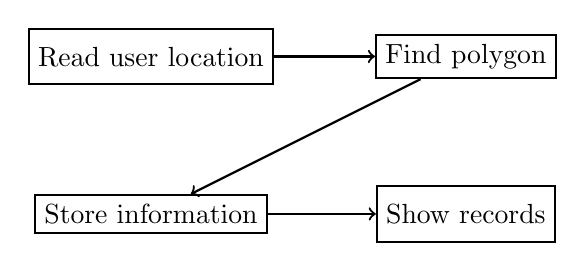
\begin{tikzpicture}[thick]
       \node[draw,rectangle,minimum size=20] (a) {Read user location};
        \node[draw,rectangle,minimum size=6,right of= a, node distance=4cm] (b) {Find polygon};
        \node[draw,rectangle,minimum size=5,below of= a, node distance=2cm] (c) {Store information};
        \node[draw,rectangle,minimum size=20,right of=c, node distance=4cm] (d) {Show records};
        \draw[->] (a) to (b);
       \draw[->,] (b) to (c);
       \draw[->] (c) to (d);
  
     \end{tikzpicture}
     \caption{Collecting user location}
   \end{figure}


Esta funcionalidad es la mas relevante de la herramienta Aire guru, ya que para otras plataformas, esta funcionalidad no es
posible si no se usan dispositivos de mediciones a nivel de usuario, es decir, el usuario tiene que llevar siempre consigo 
una estacion de medida que monitoria los diferentes agentes contaminantes.\\

\begin{figure}[ht]
    \centering
    \includegraphics[width=8cm]{importedDataDecember}
    \caption{Personal Records. December}
\end{figure}

Como somos conscientes de que usuario quizas haya empezado a utilizar la aplicacion y no tenga datos pasados disponibles,
se le ofrece la posibilidad de importar el historico de localizacion de Google, de esta manera, sera capaz de visualizar
la exposicion a la polucion desde principios del 2018 incluso si no ha estado utilizando la herramienta.  

Tendremos que tener en cuenta que para realizar la lectura de la posicion de usuario y almacenar sus datos, deberemos de 
contar con su permiso explicito e implementar un mecanismos que nos proporcione la seguridad necesaria para no poner en 
riesgo los datos de nuestros usuarios. Las medidas tomadas, se explicaran mas adelante.
 
\elsparagraph{Evaluation}  
\begin{itemize}
    \done El usuario cuenta con funcionalidades especializadas 
    \done Funcionalidad unica, el usuario es capaz de ver la polucion a la que ha estado expuesto desde 2018 incluso
    sin haber estado utilizando la herramienta
    \crossed La funcion del filtrado de la condicion medica no se autoselecciona, esto es debido a que la funcionalidad
    esta disponible para todos los usuarios. Podria implementarse de manera que el mapa mostrara el AQI con respecto a los
    contaminantes que el usuario ha preseleccionado, pero esto puede llegar a desvirtualizar la informacion si no se 
    indica al usuario claramente, que el mapa no toma en cuenta todos los contaminantes relevantes.
\end{itemize}
 \newpage